% Structure draft: section titles, preserved equations and figures.
% Karp et al. (1977) supplied expansion-opacity and Rosseland-mean formulae
% and numerical calculations. The present emphasis is transport validation
% and the representative opacity inferred from the kilonova diffusion region.
\documentclass[final,5p,times,twocolumn]{elsarticle}

\usepackage{amssymb}
\usepackage{amsmath}
\usepackage{url}
\usepackage[colorlinks=true, urlcolor=blue, linkcolor=blue, citecolor=blue]{hyperref}

\makeatletter
\setlength{\@fptop}{0pt}
\setlength{\@fpbot}{0pt plus 1fil}
\makeatother

\DeclareRobustCommand{\secref}[1]{\hyperref[#1]{Section~\ref*{#1}}}
\DeclareRobustCommand{\figref}[1]{\hyperref[#1]{Figure~\ref*{#1}}}
\DeclareRobustCommand{\eqnref}[1]{\hyperref[#1]{Eq.~(\ref*{#1})}}

\renewcommand{\ttdefault}{lmtt}
\journal{High Energy Density Physics}

\begin{document}
\begin{frontmatter}

\author[1]{Roy G. Yaron}
\cortext[cor1]{Corresponding author: \href{mailto:udini@tauex.tau.ac.il}{udini@tauex.tau.ac.il}}
\affiliation[1]{organization={School of Physics and Astronomy, Tel Aviv University},
           city={Tel Aviv}, postcode={6997801}, country={Israel}}

\title{Expansion-Aware Gray Opacities for Supernova and Kilonova Radiation Transport}

\begin{abstract}
\end{abstract}

\begin{keyword}
opacity \sep expansion opacity \sep Rosseland mean \sep kilonova \sep Type Ia supernovae
\end{keyword}
\end{frontmatter}

\section{Introduction}
\label{SecIntro}

\section{Expansion Opacity and Rosseland Averaging}
\label{SecExpansion}

\subsection{Expansion Opacity}
1. How kappa is constructed in Karp's work.
2. Check if I want to have slightly different implemntion due to practical reasons. 
(Maybe) Show its accurate enogh to use Pinto and Eastman formalism even for rosseland as long as we use low amount of bins.

\subsection{Numerical Construction and Frequency Convergence}

\begin{figure}[h]
    \centering
    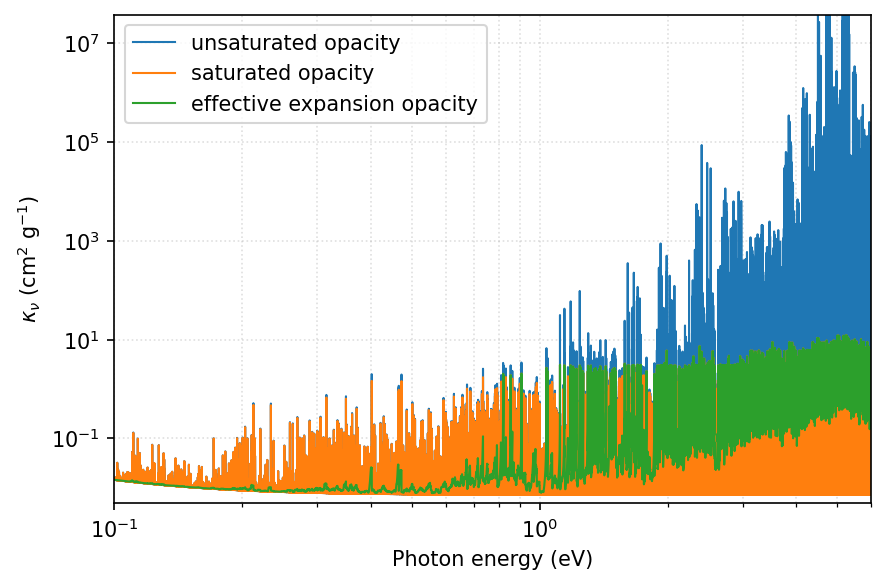
\includegraphics[width=\columnwidth]{figs/kappa_smoothed_vs_raw.png}\\[0.5em]
    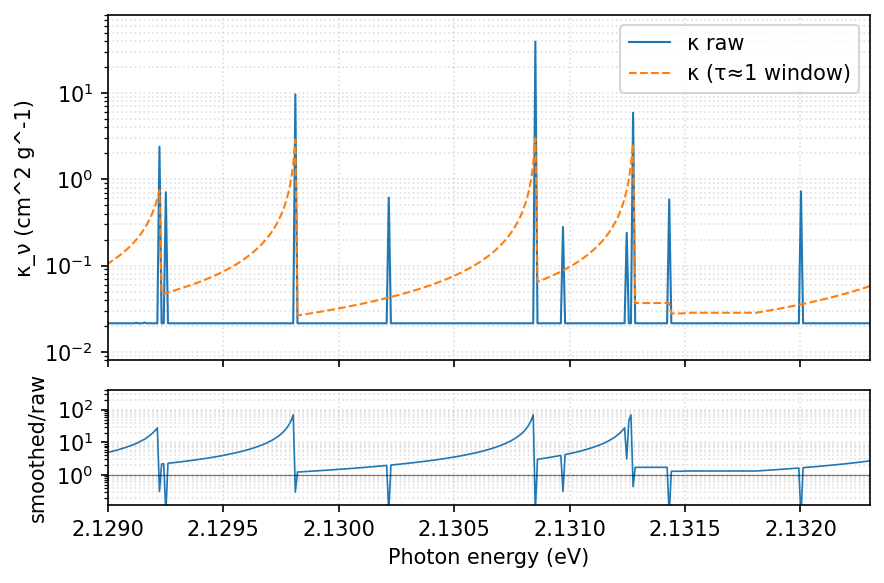
\includegraphics[width=\columnwidth]{figs/kappa_smoothed_vs_raw_error.png}
    \caption{Illustrates unsaturated, saturated, and effective expansion opacity
    for a single thermodynamic point (Fe example).}
    \label{fig:BB_line_example}
\end{figure}

\begin{figure}[h]
    \centering
    \includegraphics[width=\columnwidth]{figs/convergence_Fe_rho1.00e-13_t20.0days.png}\\[0.5em]
    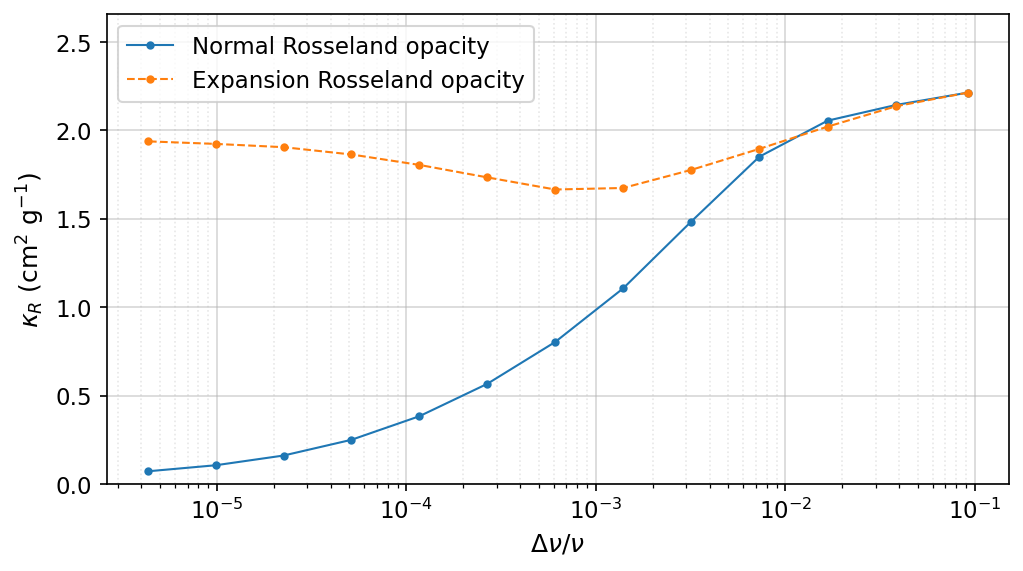
\includegraphics[width=\columnwidth]{figs/convergence_Er_rho1.00e-12_t1.0days.png}
    \caption{Convergence of $\kappa_R^{\rm exp}$ vs frequency resolution for Fe and Er.
    Shows that the gray expansion mean is numerically stable for practical binning.}
    \label{fig:convergence}
\end{figure}

\subsection{Atomic Data and Compositions}
\label{SecTables}

\begin{figure}[h]
    \centering
    \includegraphics[width=\columnwidth]{figs/kilonova_composition.png}
    \caption{Eight-element kilonova mix from solar $r$-process residuals.}
    \label{fig:kilonova_composition}
\end{figure}

\subsection{Transport Implementation and Ejecta Models}
\label{SecTransportSetup}

\section{Accuracy and Efficiency of the Gray Treatment}
\label{SecRadiationSimulations}

\subsection{Type Ia and Kilonova Bolometric Light Curves}

\begin{figure*}[t]
    \centering
    \includegraphics[width=\textwidth]{figs/luminosity_models.png}
    \caption{Single-group vs multigroup bolometric
    luminosity for SN~Ia and for kilonova $X_{\rm lan}$ series.}
    \label{fig:comparison}
\end{figure*}

\subsection{Characteristic Radiation Temperatures}

\begin{figure}[t]
    \centering
    \includegraphics[width=\columnwidth]{figs/trad_vs_phot.png}
    \caption{Escape-averaged $T_{\rm rad}$ (multigroup) vs plasma $T$ at
    $\tau_{\rm abs}(1+\tau_{\rm scat})=1$ (single-group).}
    \label{fig:trad_vs_phot}
\end{figure}

\subsection{Computational Cost}

\section{The Effective Opacity of Kilonova Ejecta}
\label{SecTypicalOpacity}

\subsection{Diffusion Depth and Column-Averaged Opacity}
\begin{equation}
    \label{eq:kappa_avg}
    \kappa_{\rm avg}(t)
    =
    \frac{\displaystyle\int_{v_{\rm diff}}^{v_{\rm max}}
        \kappa_R^{\rm exp}\,\rho\,t\,dv}
         {\displaystyle\int_{v_{\rm diff}}^{v_{\rm max}}\rho\,t\,dv}
    =
    \frac{\tau(v_{\rm diff})}{\Sigma(v_{\rm diff})}.
\end{equation}

\subsection{Thermodynamic Evolution and the Emergence of Lanthanide Dependence}

\begin{figure*}[t]
    \centering
    \includegraphics[width=\textwidth,height=0.72\textheight,keepaspectratio]{figs/kilonova_diffusion_surface.png}
    \caption{Diffusion-surface $v$, $T$, $\rho$, and
    $\kappa_{\rm avg}(t)$ for six $X_{\rm lan}$; Type~Ia local $\kappa$ panel included.}
    \label{fig:kilonova_diffusion_surface}
\end{figure*}

\begin{figure*}[t]
    \centering
    \includegraphics[width=\textwidth,height=0.36\textheight,keepaspectratio]{figs/kappa_composition_slices.png}
    \caption{Mixture $\kappa_R^{\rm exp}(T)$ and $\kappa_R^{\rm exp}(\rho)$ slices.}
    \label{fig:kappa_composition_slices}
\end{figure*}

\subsection{Representative Opacities Across Compositions and Ejecta Profiles}

\begin{figure*}[!t]
    \centering
    \includegraphics[width=\textwidth,height=0.36\textheight,keepaspectratio]{figs/kappa_vs_xlan.png}
    \caption{$\kappa_{\rm avg}$ vs $X_{\rm lan}$ for five ejecta profiles + fit.}
    \label{fig:kappa_xlan}
\end{figure*}

\subsection{A Composition-Dependent Opacity Prescription and Its Light-Curve Implications}
\begin{equation}
    \label{eq:kappa_xlan}
    \boxed{
    \kappa_{\rm avg}(X_{\rm lan})
    =
    0.34 + 99\,X_{\rm lan}^{0.72}\ {\rm cm^{2}\,g^{-1}}.
    }
\end{equation}

\section{Discussion and Conclusions}
\label{SecSummary}

\appendix

\section{Frequency-Bin Interpolation and Limiting Cases}
\label{AppInterpolation}

\begin{equation}
    \kappa_{\rm bb}^{\rm sat}(\nu)
    = \sum_l \frac{\nu_l}{\rho c t}\,\delta(\nu-\nu_l)\,(1-e^{-\tau_l}),
\end{equation}
\begin{equation}
    \kappa_{\rm bb}^{\rm unsat}(\nu)
    = \sum_l \frac{\nu_l}{\rho c t}\,\delta(\nu-\nu_l)\,\tau_l .
\end{equation}

\begin{equation}
    \label{eq:kappa_eff}
    \kappa_{\rm exp}(\nu_i)
    = \frac{\sum_l (1-e^{-\tau_l})}{\rho\,c t\,\ln(\nu_{i+1}/\nu_i)}
      + \kappa_{\rm T} + \kappa_{\rm ff}(\nu_i).
\end{equation}

\section{Opacity Maps and Comparison with Planck Means}
\label{AppOpacityMaps}

\begin{figure*}[t]
    \centering
    \includegraphics[width=0.48\textwidth]{figs/ni_rosseland_t1d.png}\hspace{0.02\textwidth}%
    \includegraphics[width=0.48\textwidth]{figs/ni_t1d_ratio.png}
    \caption{SN~Ia core: $\kappa_R^{\rm exp}$ and $\kappa_P/\kappa_R^{\rm exp}$ at $t=1$~d.}
    \label{fig:rosseland_planck_ni}
\end{figure*}

\begin{figure*}[t]
    \centering
    \includegraphics[width=0.48\textwidth]{figs/sn1a_outer_rosseland_t1d.png}\hspace{0.02\textwidth}%
    \includegraphics[width=0.48\textwidth]{figs/sn1a_outer_ratio_t1d.png}
    \caption{SN~Ia outer layer: same quantities at $t=1$~d.}
    \label{fig:rosseland_planck_sn1a_outer}
\end{figure*}

\begin{figure*}[t]
    \centering
    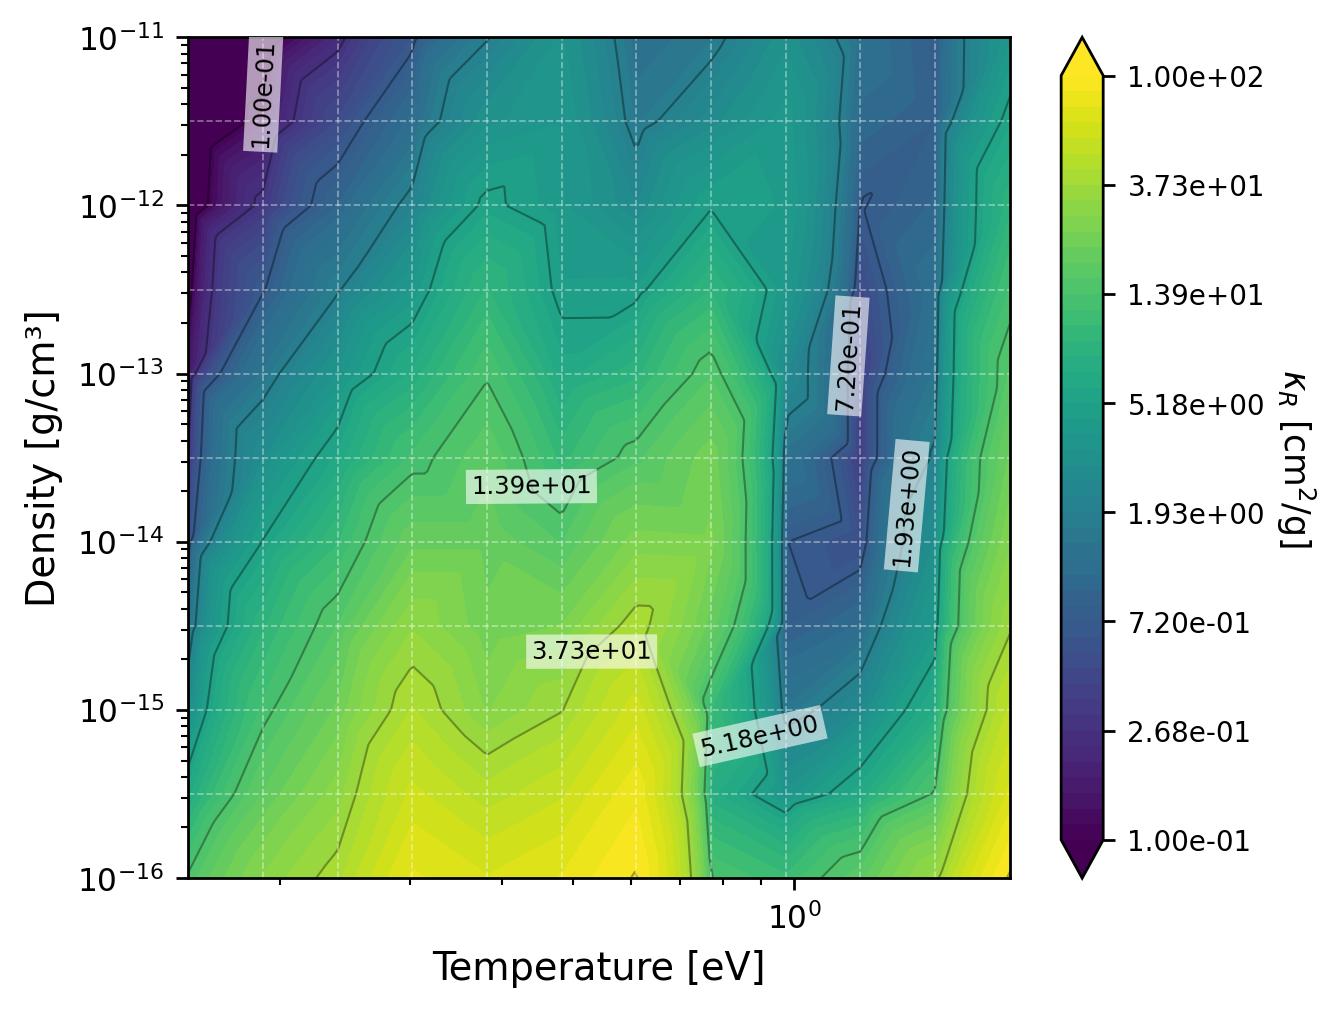
\includegraphics[width=0.48\textwidth]{figs/kilonova_rosseland_t1d.png}\hspace{0.02\textwidth}%
    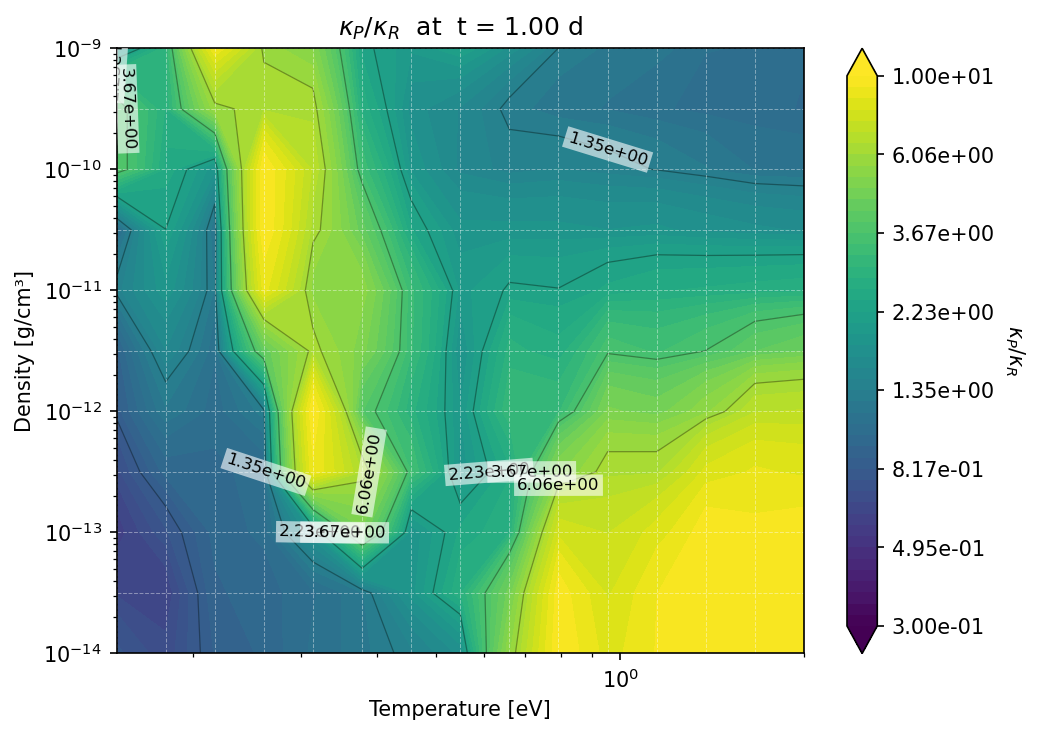
\includegraphics[width=0.48\textwidth]{figs/kilonova_ratio_t1d.png}
    \caption{Kilonova mix ($X_{\rm lan}=0.121$): same quantities at $t=1$~d.}
    \label{fig:rosseland_planck_kilonova}
\end{figure*}

\begin{figure*}[t]
    \centering
    \includegraphics[width=\textwidth]{figs/profile_colormap_dreff_compare.png}
    \caption{SN~Ia $T_{\rm plasma}$ and $\kappa_R^{\rm exp}$ maps with diffusion /
    photosphere surfaces overlaid.}
    \label{fig:profile_colormap}
\end{figure*}

\section{Individual-Lanthanide Opacities and Ionization Features}
\label{AppLanthanides}

\begin{figure*}[t]
    \centering
    \includegraphics[width=\textwidth]{figs/all_lanthanides_opacity.pdf}
    \caption{All-lanthanide $\kappa_R$ and $\kappa_P$ vs $T$; documents
    the $\sim1.2$~eV feature as database-wide for high-opacity lanthanides.}
    \label{fig:all_lanthanides_opacity}
\end{figure*}

\end{document}
